\PassOptionsToPackage{hyphens}{url}
\documentclass[11pt,a4paper]{article}

%\usepackage[provide=*,spanish]{babel}
\usepackage[utf8]{inputenc}
\usepackage[spanish]{babel}
\usepackage[T1]{fontenc}
\usepackage{lmodern}
\usepackage[margin=2.35cm]{geometry}
\usepackage{amsmath}
\usepackage{booktabs}
\usepackage{longtable}
\usepackage{tabularx}
\usepackage{array}
\usepackage{enumitem}
\usepackage{listings}
\usepackage{xcolor}
\usepackage{microtype}
\usepackage{parskip}
\usepackage{titlesec}
\usepackage{hyperref}
\usepackage{graphicx}
\usepackage{caption}
\usepackage{float}

\definecolor{azulWCD}{RGB}{17,67,112}
\definecolor{grisCodigo}{RGB}{247,247,247}
\definecolor{verdeCodigo}{RGB}{25,110,55}
\definecolor{rojoCodigo}{RGB}{145,35,35}
\definecolor{tituloColor}{RGB}{0,55,110}
\definecolor{reglaColor}{RGB}{0,90,160}

\hypersetup{
  colorlinks=true,
  linkcolor=azulWCD,
  urlcolor=azulWCD,
  citecolor=azulWCD,
  pdftitle={Procesamiento reproducible de la Campana 1: 64 corridas de neutrones monoenergeticos},
  pdfauthor={Jaime A. Betancourt}
}

\lstdefinestyle{shstyle}{
  backgroundcolor=\color{grisCodigo},
  basicstyle=\ttfamily\footnotesize,
  breaklines=true,
  frame=single,
  rulecolor=\color{gray!40},
  columns=fullflexible,
  keepspaces=true
}
\lstset{style=shstyle}

\titleformat{\section}{\normalfont\Large\bfseries\color{azulWCD}}
  {\thesection.}{0.6em}{}
\titleformat{\subsection}{\normalfont\large\bfseries}
  {\thesubsection.}{0.5em}{}
\setlist{itemsep=0.25em,topsep=0.4em}
\renewcommand{\arraystretch}{1.18}
\setlength{\emergencystretch}{2em}

\newcommand{\codigo}[1]{\nolinkurl{#1}}
\newcommand{\archivo}[1]{\path{#1}}
\newcommand{\var}[1]{\texttt{#1}}

\begin{document}
\pagestyle{empty}

\begin{titlepage}
\begin{center}

\vspace*{0.5cm}
\textcolor{reglaColor}{\rule{\linewidth}{1.2pt}}

\vspace{1.3cm}
{\Large\scshape Universidad Industrial de Santander}\\[0.2cm]
{\large Escuela de Física --- Facultad de Ciencias}\\[0.2cm]
{\large Doctorado en Física}

\vspace{2.2cm}
{\Huge\bfseries\color{tituloColor} Procesamiento reproducible\\[0.2cm]
de la Campaña 1:\\[0.2cm] 64 corridas de neutrones monoenergéticos}

\vspace{1.8cm}
{\large\textbf{Informe técnico}}

\vspace{0.6cm}
\begin{minipage}{0.82\linewidth}
\centering
\textit{``De los archivos crudos del simulador a las cifras de la Sección~4.2 de la tesis: método, validación y resultados para dieciséis energías y cuatro medios''}
\end{minipage}

\vfill

{\large\textbf{Autor}}\\[0.15cm]
Jaime A. Betancourt\\[0.1cm]
Doctorado en Física, Universidad Industrial de Santander

\vspace{1.2cm}
\textcolor{reglaColor}{\rule{0.5\linewidth}{0.6pt}}

\vspace{1cm}
5 de octubre de 2026

\vspace{1cm}
\textcolor{reglaColor}{\rule{\linewidth}{1.2pt}}

\end{center}
\end{titlepage}

\pagestyle{plain}

\begin{abstract}
Este informe documenta el procesamiento de las 64 corridas de la Campaña~1 de la tesis (dieciséis energías de inyección entre 1~meV y la corrida rotulada ``1~keV'', por cuatro medios: agua pura y soluciones con 2.5, 5 y 10~\% de NaCl en masa; 100\,000 neutrones por corrida, física \texttt{QGSP\_BERT\_HP} sin $S(\alpha,\beta)$). Dos scripts del repositorio leen solo las salidas crudas del simulador y producen, en una sola pasada y en alrededor de un minuto para toda la campaña, una tabla por neutrón y un resumen por corrida. El procesamiento reproduce exactamente el análisis original: el balance de destinos coincide en las 64 corridas con el de la Tabla~4.8 y el Apéndice~C, los conteos por proceso y por historia son idénticos a los archivos originales, y el número medio de dispersiones elásticas antes de la captura, $\langle N\rangle$, reproduce los valores citados (44.78 a 1~meV y 76.78 a 1~keV en agua pura). La letargía $\xi$ se calcula con la definición de la tesis, por colisión, que reemplazó a la definición inicial por historia del estudio; el informe documenta esa diferencia, señala un redondeo corregido en la tesis, recalcula la longitud de captura de la Tabla~4.9 y verifica que seleccionar los pasos con un cilindro en lugar de una caja cuadrada no modifica los resultados.
\end{abstract}

\tableofcontents

\section{Objeto y alcance}

Los resultados de la Sección~4.2 de la tesis (respuesta del WCD a neutrones monoenergéticos) se obtuvieron originalmente con notebooks ejecutados carpeta por carpeta, que generaban numerosos archivos intermedios. Este informe describe un procesamiento nuevo, automatizado y verificable, cuyo propósito es:

\begin{enumerate}
  \item reconstruir todas las magnitudes por neutrón y por corrida a partir de los archivos crudos, sin archivos intermedios;
  \item verificar que las cifras publicadas en la tesis se reproducen con ese procesamiento;
  \item dejar el método documentado en el repositorio, como base del notebook que regenerará las figuras de la Sección~4.2.
\end{enumerate}

Este informe reemplaza al informe anterior de la misma carpeta (\archivo{Informe-tecnico-Analisis-Moderacion-Captura-Neutrones}), que analizaba cinco energías con otro conjunto de datos y clasificaba los destinos por las caras de la caja del mundo de Geant4. La clasificación por caras del volumen activo empleada aquí es la de la versión final de la tesis.

\section{Datos de entrada}
\label{sec:datos}

Las corridas se encuentran en la carpeta \archivo{Neutrones-termicos/energia/medio/} del equipo del autor. Las dieciséis energías son 1, 2.5, 5, 7, 10, 25, 50, 80, 100, 300, 500 y 700~meV y las carpetas \codigo{1000meV}, \codigo{10000meV}, \codigo{100000meV} y \codigo{1000000meV}, rotuladas en la tesis como 1~eV, 10~eV, 100~eV y 1~keV. Los medios son \codigo{Agua-pura}, \codigo{Agua+2.5NaCl}, \codigo{Agua+5NaCl} y \codigo{Agua+10NaCl}. Las 64 carpetas contienen los mismos archivos crudos:

\begin{center}
\begin{tabularx}{\linewidth}{@{}lX@{}}
\toprule
\textbf{Archivo} & \textbf{Contenido} \\
\midrule
\archivo{interaccion-completa-neutrones.txt} & Un paso del neutrón primario por línea: número de paso, partícula, \textit{track}, padre, $E_\mathrm{pre}$ [MeV], posición previa $(x_0,y_0,z_0)$ y posterior $(x_1,y_1,z_1)$ [mm], $E_\mathrm{post}$ [MeV] y proceso. Una historia empieza cuando el número de paso vuelve a 1. \\
\archivo{neutrones-capturados.txt} & Posición y energía de cada captura. Se usa solo para verificar. \\
\archivo{Carga_Total_*.txt} & Número de fotoelectrones de cada evento con señal en el PMT. \\
\bottomrule
\end{tabularx}
\end{center}

El archivo de partículas secundarias de la captura (\archivo{secondary-particles-neutron-capturado.txt}) solo existe en la carpeta de 1~meV en agua pura; los espectros gamma de la tesis provienen de otro conjunto de datos y no forman parte de este procesamiento.

\textbf{Verificación de la inyección.} En las 64 corridas, la primera línea registra la posición inicial $z_0 = 1500$~mm, coincidente con la inyección vertical desde 1.5~m descrita en la tesis, y una energía $E_0$ igual al valor nominal de la carpeta. 
%En la carpeta \codigo{1000000meV}, $E_0 = 9.99997\times10^{-3}$~MeV; esta corrida se rotula ``1~keV'' en la tesis por decisión del autor, y ese rótulo se conserva en las figuras de este informe.

\section{Método}
\label{sec:metodo}

\subsection{Procesamiento en una sola pasada}

El script \archivo{procesar_corrida.py} recorre \archivo{interaccion-completa-neutrones.txt} una sola vez. Para cada historia acumula sus pasos y, al cerrarla, calcula todas las magnitudes; en paralelo alimenta la máquina de estados que reproduce la definición de $N$ de la tesis (Sección~\ref{sec:N}). El script \archivo{procesar_campana.py} lo ejecuta sobre las 64 corridas en paralelo y reúne los resúmenes.

\subsection{Destino final de cada neutrón}

Cada historia se clasifica según la última frontera del volumen activo ($|x|,|y|\le 480$~mm, $0\le z\le 1330$~mm) que atraviesa, igual que en el script \archivo{balance_caras_tanque.py} de la revisión final de la tesis. Las categorías son captura dentro o fuera del volumen activo, salida por la tapa (reflexión), salida por el fondo o por las paredes laterales (transmisión) y otros destinos (no ingresa al volumen activo o termina en una interacción inelástica). Los coeficientes $\eta$ se dan con su incertidumbre binomial $\sqrt{\eta(1-\eta)/N_\mathrm{inc}}$.

\subsection{Número de dispersiones elásticas antes de la captura, $N$}
\label{sec:N}

Se conserva la definición del notebook original, que es la usada en la tesis:

\begin{enumerate}
  \item se seleccionan los pasos con la posición previa o la posterior dentro de la caja $|x|,|y|\le478$~mm y $0\le z\le1330$~mm;
  \item en esa secuencia se busca una cadena que empiece en una dispersión elástica (\var{hadElastic}), continúe solo con dispersiones elásticas en pasos consecutivos y termine en una captura;
  \item $N$ es el número de dispersiones elásticas de la cadena. Una captura sin dispersiones previas dentro de la caja cuenta como $N = 0$.
\end{enumerate}

Una historia capturada cuya cadena se interrumpe (por ejemplo, porque el neutrón sale de la caja y vuelve a entrar) no aporta un valor de $N$. A 1~meV en agua pura, la cadena es válida en 17\,213 de las 17\,418 capturas. Como verificación se guarda también $N_\mathrm{total}$, el número de todas las dispersiones elásticas de la historia capturada, que da $\langle N_\mathrm{total}\rangle = 44.62$ frente a $\langle N\rangle = 44.78$.

\subsection{Letargía $\xi$: definición de la tesis}
\label{sec:xi}

En la tesis, $\xi$ es la letargía de cada dispersión elástica,
\[
\xi = \ln\!\left(\frac{E_\mathrm{pre}}{E_\mathrm{post}}\right),
\]
calculada para las dispersiones elásticas de las cadenas válidas de la Sección~\ref{sec:N}, es decir, de las cadenas ininterrumpidas que terminan en captura, como en los notebooks \archivo{Histogramas_cita_*.ipynb} que generaron las Figuras~4.20--4.23 y D.4--D.6. $\langle\xi\rangle$ y $\sigma(\xi)$ se toman sobre todas esas colisiones, y las figuras usan un histograma de 300 intervalos entre $-2$ y $2$ normalizado a área unitaria. A 1~meV en agua pura son 770\,803 colisiones, igual a $17\,213\times\langle N\rangle$. Con esta definición están calculados los resultados y el análisis de la tesis; por ejemplo, $\langle\xi\rangle$ = 0.058 a 1~eV y 0.165 a 1~keV en agua pura (Figura~4.23 y Capítulo~5). El procesamiento guarda por corrida el número de colisiones, $\langle\xi\rangle$, $\sigma(\xi)$ y el histograma, y por historia la suma de $\xi$ de su cadena.

\textbf{Definición inicial, reemplazada.} En sus inicios, el estudio calculaba $\xi$ por historia, $\xi_\mathrm{ini} = \ln(E_0/E_\mathrm{cap})/N$, con $E_0$ la energía antes de la primera dispersión de la cadena, $E_\mathrm{cap}$ la energía antes de la captura y $N$ el número de dispersiones, y lo promediaba sobre historias. Esa definición se corrigió y fue reemplazada por la anterior; es la que conservan los notebooks antiguos de las carpetas de datos. Tiene el mismo signo que el $\xi$ por colisión, pero su magnitud es apreciablemente mayor (Figura~\ref{fig:xi}). Este procesamiento la conserva solo por trazabilidad, en la columna \var{xi\_historia\_inicial}, y para validar que reproduce exactamente los archivos de los notebooks antiguos.

\subsection{Carga}

Para cada corrida se registran el número de eventos con señal y la media de fotoelectrones por evento, leídos directamente de \archivo{Carga_Total_*.txt}.

\subsection{Salidas}

\begin{center}
\begin{tabularx}{\linewidth}{@{}lX@{}}
\toprule
\textbf{Archivo} & \textbf{Contenido} \\
\midrule
\archivo{historias.tsv.gz} & Una fila por neutrón: número de pasos y conteos de \var{Transportation}, \var{hadElastic}, \var{neutronInelastic} y \var{nCapture}; último proceso; destino; posición y energía de captura; $N_\mathrm{total}$ y $N$; la suma de $\xi$ en las dispersiones elásticas de la cadena, y $\xi_\mathrm{ini}$ (definición inicial, solo para trazabilidad). Entre 1.4 y 2.2~MB por corrida. \\
\archivo{resumen.json} & Medias por historia, destinos, coeficientes $\eta$ con incertidumbre, $\langle N\rangle$ y el histograma de $N$, $\langle\xi\rangle$, $\sigma(\xi)$ y el histograma de $\xi$ de la tesis (y, por trazabilidad, el $\langle\xi\rangle$ de la definición inicial), y la estadística y el histograma de la carga. \\
\archivo{resumen_campana.tsv} & Una fila por corrida con todas las magnitudes anteriores. \\
\bottomrule
\end{tabularx}
\end{center}

\section{Validación}
\label{sec:validacion}

\begin{center}
\begin{tabularx}{\linewidth}{@{}Xll@{}}
\toprule
\textbf{Comprobación} & \textbf{Alcance} & \textbf{Resultado} \\
\midrule
Coeficientes de captura, reflexión, transmisión y otros frente a \archivo{balance_caras_tanque.tsv} (Tabla~4.8 y Apéndice~C) & 64 corridas & idénticos \\
Conteo de \var{hadElastic} por historia frente a los archivos \archivo{hadElastic-*.txt} originales & 15 corridas que los conservan & idénticos \\
Conteos por historia de los cuatro procesos (1~meV, agua pura) & 100\,000 historias & idénticos \\
Valores de $N$ y $\xi_\mathrm{ini}$ frente a los archivos del notebook antiguo (1~meV, agua pura) & 17\,213 cadenas & idénticos y en el mismo orden \\
Posiciones de captura frente a \archivo{neutrones-capturados.txt} (1~meV, agua pura) & 17\,418 capturas & idénticas \\
\bottomrule
\end{tabularx}
\end{center}

Las cifras de la Campaña~1 que cita el Capítulo~5 se reproducen todas:

\begin{center}
\small
\begin{tabularx}{\linewidth}{@{}l>{\raggedright\arraybackslash}Xrr@{}}
\toprule
\textbf{Magnitud} & \textbf{Corrida} & \textbf{Procesamiento} & \textbf{Tesis} \\
\midrule
$\langle N\rangle$ & 1~meV / 25~meV / 1~eV / 1~keV, agua pura & 44.78 / 52.15 / 60.41 / 76.78 & 44.8 / 52.2 / 60.4 / 76.8 \\
$\eta_\mathrm{Cap}$ & 1~meV, agua pura & $(17.418\pm0.120)$~\% & $(17.42\pm0.12)$~\% \\
$\eta_\mathrm{Cap}$ & 1~eV, agua pura / 10~\% NaCl & 35.88 / 51.38~\% & 35.88 / 51.38~\% \\
$\eta_\mathrm{Cap}$ & 1~keV, agua pura & 33.77~\% & 33.77~\% \\
$\eta_\mathrm{Refle}$ & 1~meV / 1~eV / 1~keV, agua pura & 76.57 / 62.17 / 64.56~\% & 76.6 / 62.2 / 64.6~\% \\
Captura relativa & 1~meV; 10, 5, 2.5~\% NaCl & 1.614 / 1.346 / 1.185 & 1.61 / 1.35 / 1.19 \\
Captura relativa & 1~keV; 10, 5, 2.5~\% NaCl & 1.345 / 1.212 / 1.112 & 1.35 / 1.21 / 1.11 \\
$\langle\xi\rangle$ & 1~eV / 1~keV, agua pura & 0.0583 / 0.1651 & 0.058 / 0.165 \\
\bottomrule
\end{tabularx}
\end{center}

Un valor de la tesis no correspondía al redondeo correcto: la captura relativa a 1~keV con 10~\% de NaCl es 1.3447, que redondea a 1.34 y no a 1.35. La diferencia es menor que la incertidumbre estadística; el valor ya se corrigió en los Capítulos~4 y~5.

Además, para las 64 corridas, el número de colisiones, $\langle\xi\rangle$ y $\sigma(\xi)$ coinciden con los valores impresos por los notebooks \archivo{Histogramas_cita_*.ipynb}, y la tabla de la Figura~4.19 ($x_\mathrm{max}$, FWHM y $\langle N\rangle$ de las siete energías) se reproduce exactamente. Los promedios de pasos por neutrón de las Figuras~4.17 y 4.18 coinciden en 61 de las 64 corridas; en tres corridas (700~meV con 2.5 y 5~\% de NaCl y 10~eV con 2.5~\%) el archivo de promedios que usaron esas figuras difiere de los datos crudos actuales hasta en 0.7~\% (también en la captura), aunque los histogramas de $\xi$ de esas mismas corridas sí coinciden. Esos tres puntos se calcularon, por tanto, con otra copia de los datos.

\section{Resultados}
\label{sec:resultados}

\subsection{Balance de destinos}

\begin{figure}[H]
  \centering
  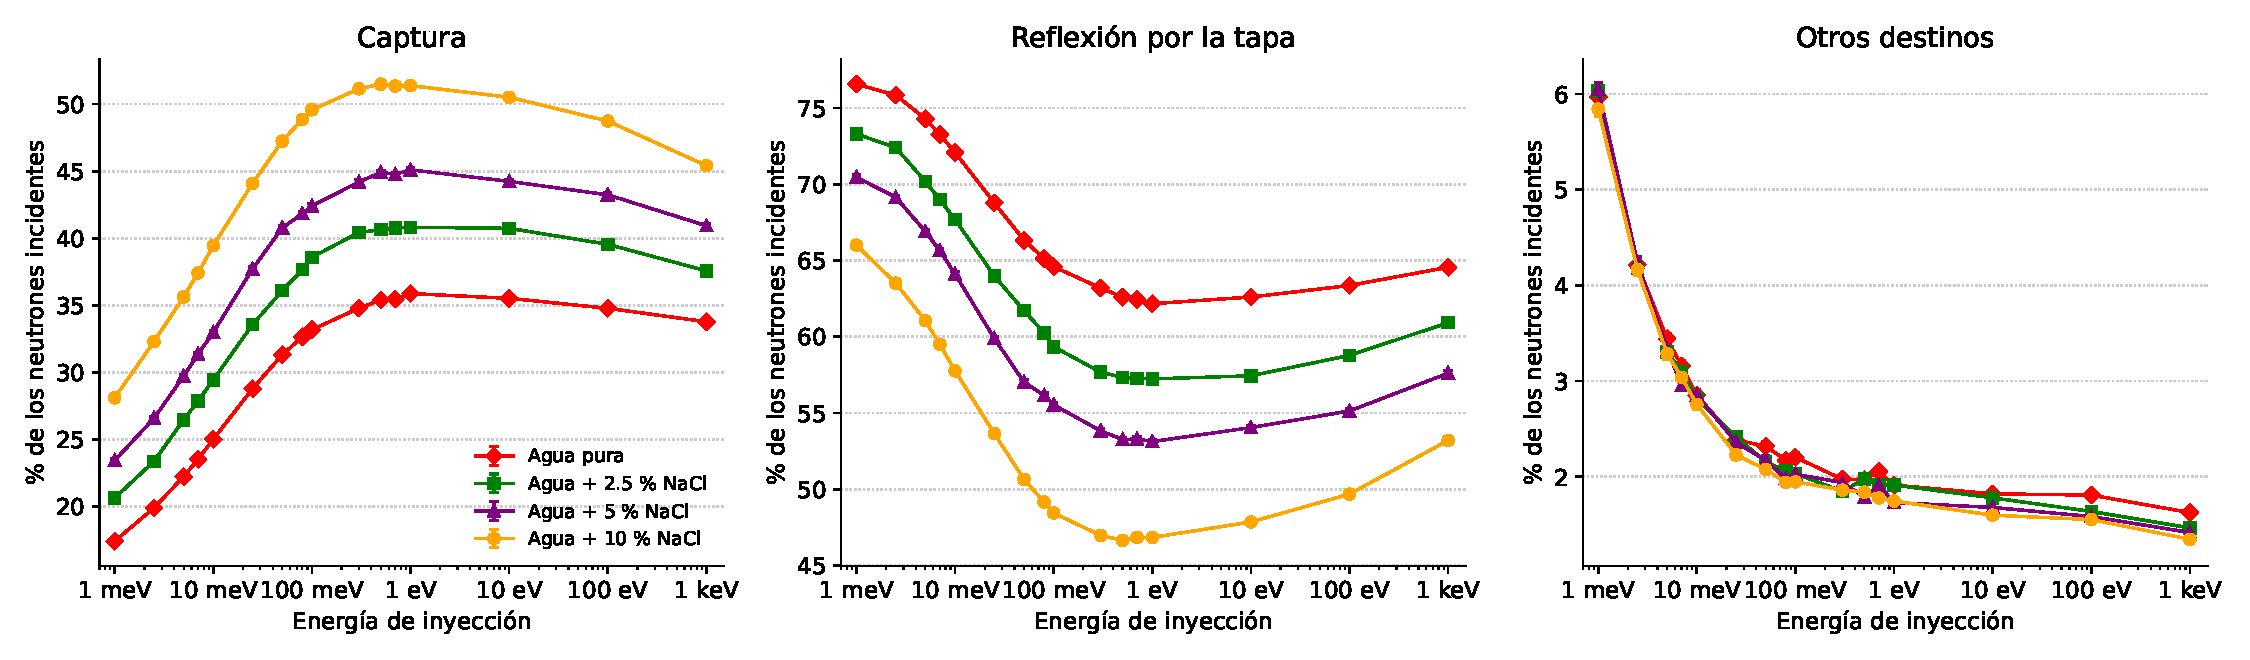
\includegraphics[width=\linewidth]{figuras-procesamiento-64-corridas/balance_destinos.pdf}
  \caption{Fracción de neutrones capturados, reflejados por la tapa y con otros destinos, en función de la energía de inyección. Las barras de error ($1\sigma$, binomiales) son menores que los símbolos. La transmisión por el fondo y las paredes laterales no se muestra: está entre 0.02 y 0.06~\% en todas las corridas.}
  \label{fig:balance}
\end{figure}

La captura presenta un máximo amplio entre 0.3~eV y 10~eV y disminuye hacia las energías frías y hacia 1~keV; el NaCl la aumenta en las dieciséis energías. Casi todo ese aumento se produce a expensas de la reflexión por la tapa, porque la transmisión es despreciable y la fracción de otros destinos (de 6~\% a 1~meV a menos de 2~\% por encima de 1~eV) casi no depende del medio. Entre 0.07 y 1.6~\% de las capturas ocurre fuera del volumen activo, en la estructura del tanque.

\subsection{Pasos por historia}

\begin{figure}[H]
  \centering
  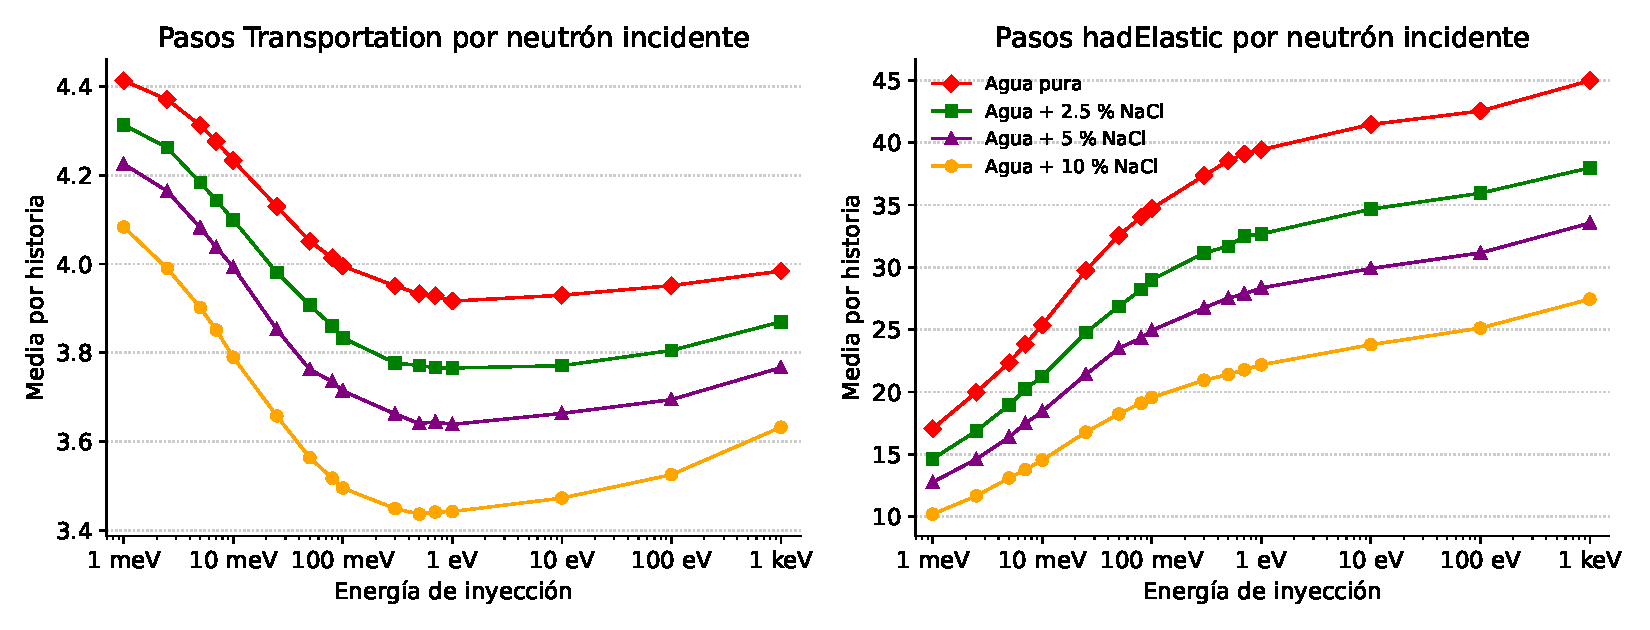
\includegraphics[width=\linewidth]{figuras-procesamiento-64-corridas/pasos_por_historia.pdf}
  \caption{Número medio de pasos \var{Transportation} y \var{hadElastic} por neutrón incidente (todas las historias), base de las Figuras~4.17 y 4.18 de la tesis.}
  \label{fig:pasos}
\end{figure}

\subsection{Dispersiones elásticas antes de la captura}

\begin{figure}[H]
  \centering
  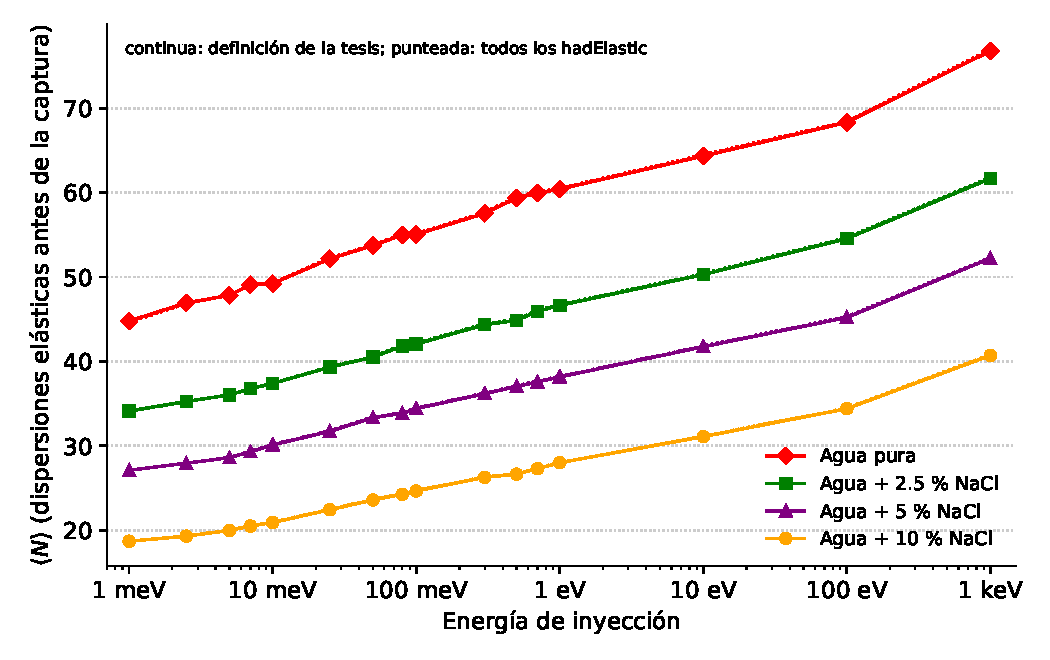
\includegraphics[width=0.78\linewidth]{figuras-procesamiento-64-corridas/N_medio.pdf}
  \caption{$\langle N\rangle$ en función de la energía de inyección. Línea continua: definición de la tesis; línea punteada: todas las dispersiones elásticas de la historia capturada. Las dos definiciones difieren en menos del 0.5~\%.}
  \label{fig:N}
\end{figure}

\begin{figure}[H]
  \centering
  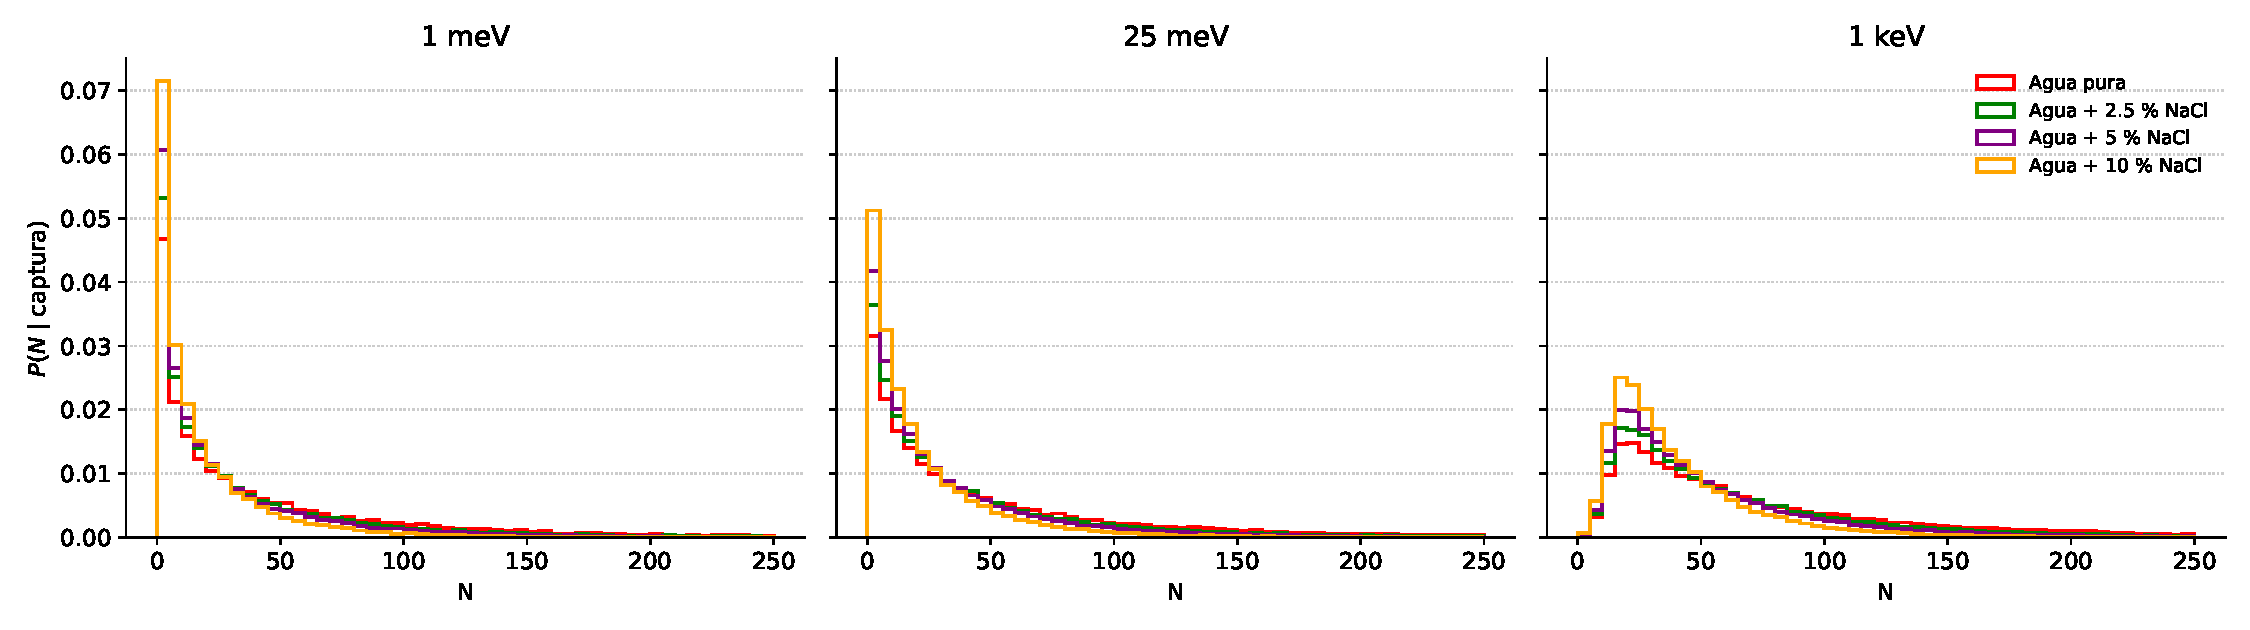
\includegraphics[width=\linewidth]{figuras-procesamiento-64-corridas/N_distribuciones.pdf}
  \caption{Distribución $P(N\mid\text{captura})$ a 1~meV, 25~meV y 1~keV para los cuatro medios. El primer intervalo incluye las capturas con $N=0$.}
  \label{fig:Ndist}
\end{figure}

$\langle N\rangle$ crece de forma monótona con la energía en los cuatro medios y disminuye con la concentración de NaCl, porque el cloro acorta la vida del neutrón térmico antes de la captura: a 1~meV pasa de 44.8 en agua pura a 18.7 con 10~\% de NaCl, y a 1~keV, de 76.8 a 40.7.

\subsection{Letargía $\xi$}

\begin{figure}[H]
  \centering
  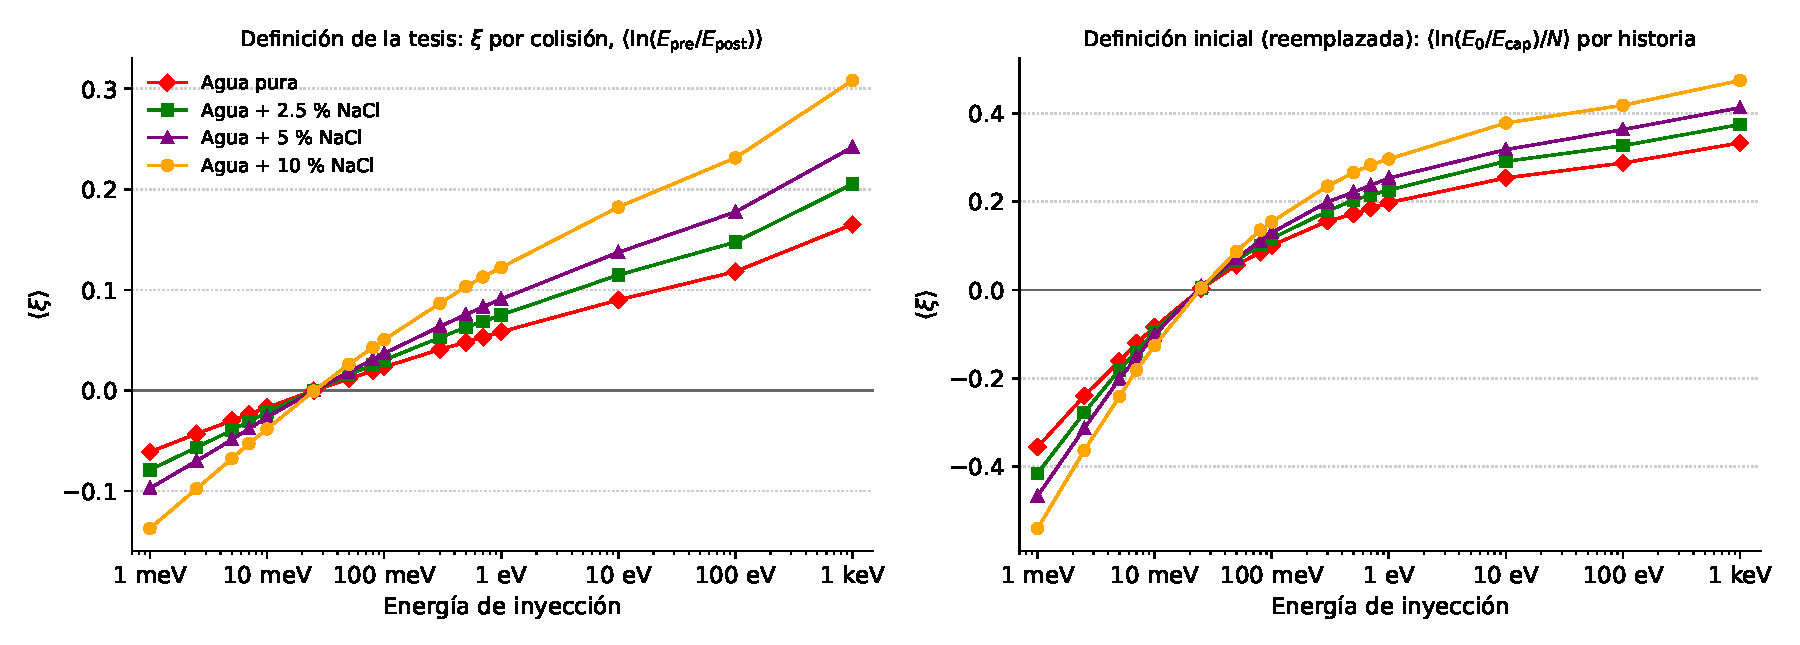
\includegraphics[width=\linewidth]{figuras-procesamiento-64-corridas/xi_medio.pdf}
  \caption{Izquierda: $\langle\xi\rangle$ con la definición de la tesis (por colisión). Derecha, solo como referencia: la definición inicial por historia, reemplazada en el estudio. Ambas cambian de signo cerca de 25~meV, la energía térmica del medio a 20~$^\circ$C.}
  \label{fig:xi}
\end{figure}

Con la definición de la tesis, por debajo de la energía térmica $\langle\xi\rangle<0$: el medio cede energía al neutrón. Por encima, $\langle\xi\rangle>0$ y crece con la energía. Con NaCl, el valor absoluto es mayor, lo que es coherente con historias capturadas más cortas, que se alejan menos de la energía inicial antes de la captura.

\subsection{Profundidad de captura}

\begin{figure}[H]
  \centering
  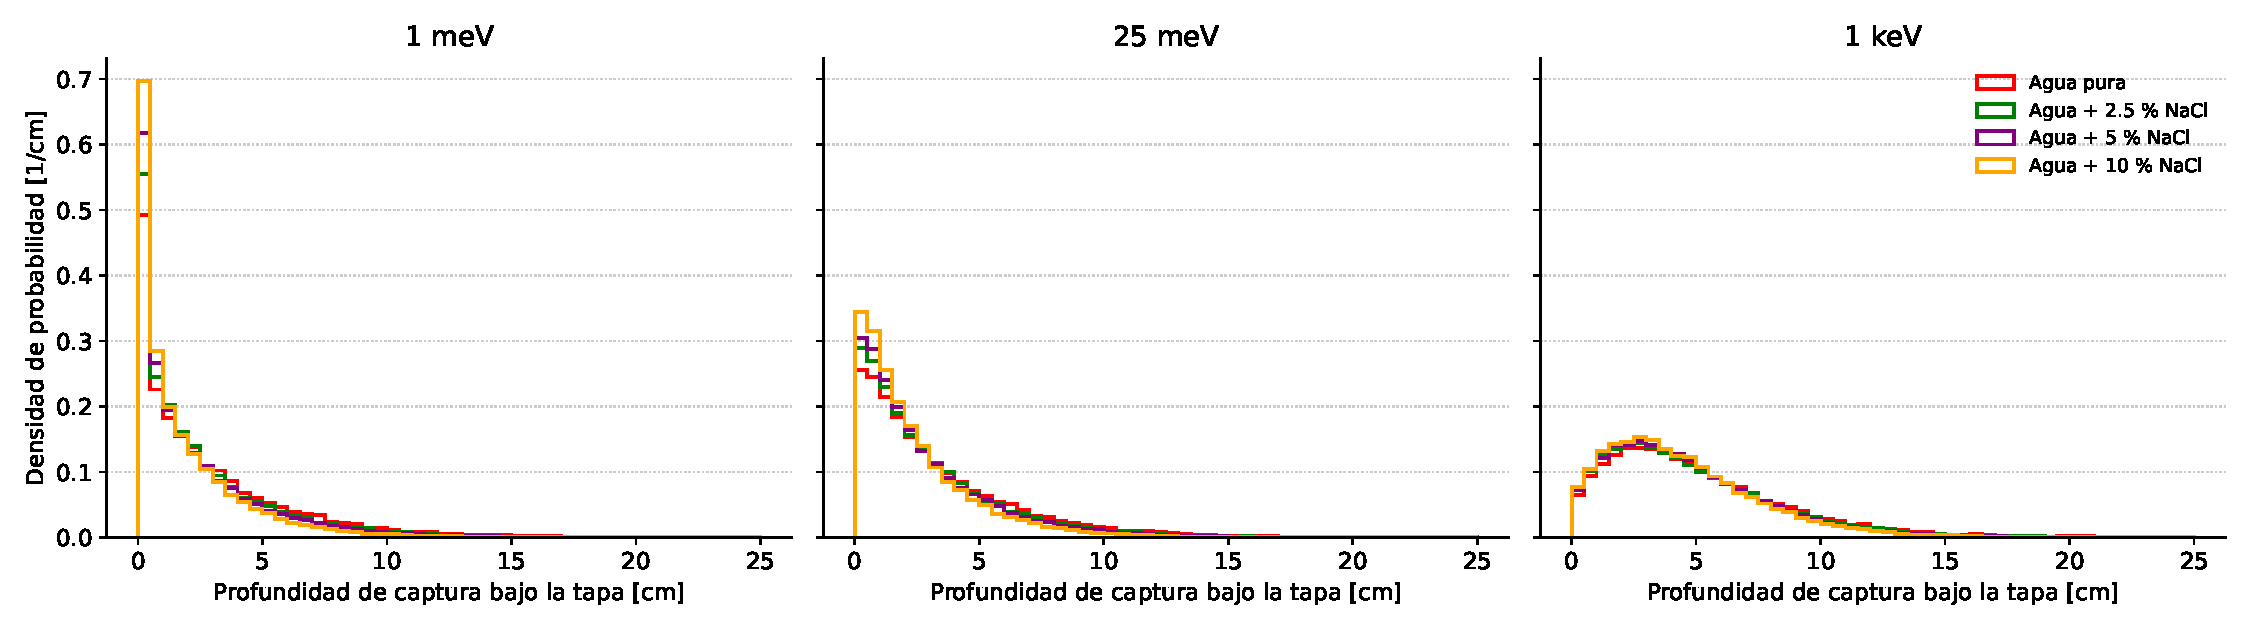
\includegraphics[width=\linewidth]{figuras-procesamiento-64-corridas/profundidad_captura.pdf}
  \caption{Profundidad de captura bajo la cara interior de la tapa ($z=1330$~mm) para las capturas dentro del volumen activo.}
  \label{fig:prof}
\end{figure}

Las capturas se concentran en los primeros centímetros bajo la tapa. En agua pura, la profundidad mediana pasa de 1.8~cm a 1~meV a 4.3~cm a 1~keV, y el 90~\% de las capturas ocurre a menos de 7--10~cm; con 10~\% de NaCl, las capturas son más superficiales (mediana de 1.0~cm a 1~meV).

\subsection{Carga}

\begin{figure}[H]
  \centering
  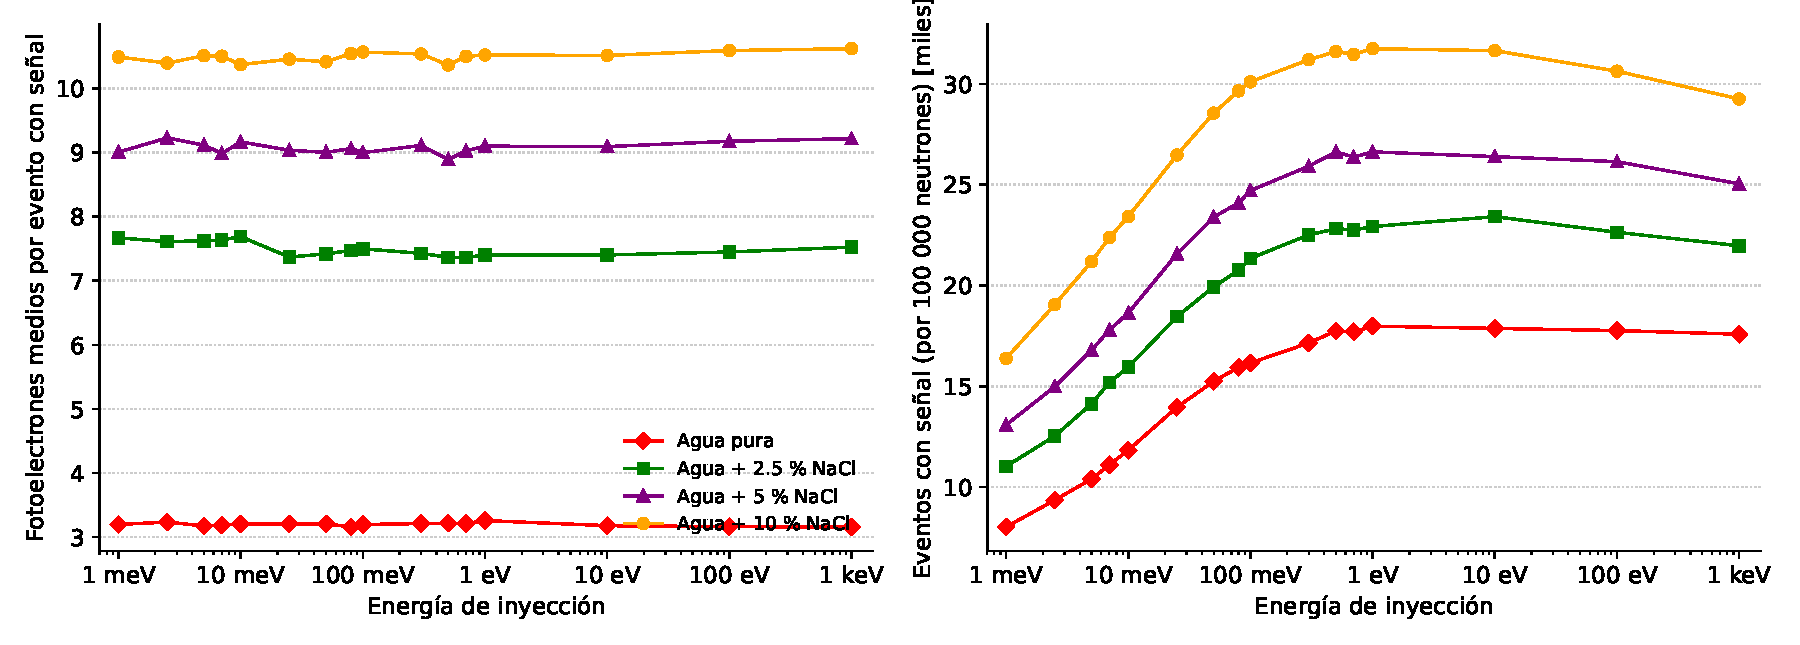
\includegraphics[width=\linewidth]{figuras-procesamiento-64-corridas/carga.pdf}
  \caption{Fotoelectrones medios por evento con señal y número de eventos con señal por cada 100\,000 neutrones inyectados.}
  \label{fig:carga}
\end{figure}

La carga media por evento con señal casi no depende de la energía de inyección, pero crece con la concentración de NaCl (de unos 3.2 a unos 10.5 fotoelectrones), por la mayor energía de la cascada gamma de la captura en $^{35}$Cl. El número de eventos con señal sigue la forma de la captura.

\subsection{Tablas por medio}

En todas las tablas, $\eta$ está en porcentaje, $\langle\xi\rangle$ es el $\xi$ de la tesis (por colisión), $\langle\xi\rangle_\mathrm{ini}$ el de la definición inicial (solo por trazabilidad) y $\bar{Q}$ la carga media en fotoelectrones por evento con señal.

\newcommand{\tablamedio}[2]{%
\begin{center}
\small
\textbf{#2}\\[0.2em]
\begin{tabular}{@{}lrrrrrrrr@{}}
\toprule
$E$ & $\eta_\mathrm{Cap}$ & $\eta_\mathrm{Refle}$ & $\eta_\mathrm{Trans}$ & $\eta_\mathrm{Otros}$ & $\langle N\rangle$ & $\langle\xi\rangle$ & $\langle\xi\rangle_\mathrm{ini}$ & $\bar{Q}$ \\
\midrule
\csname @@input\endcsname figuras-procesamiento-64-corridas/tabla_#1.tex 
\bottomrule
\end{tabular}
\end{center}}

\tablamedio{Agua-pura}{Agua pura}
\tablamedio{Agua+2.5NaCl}{Agua + 2.5~\% de NaCl}
\tablamedio{Agua+5NaCl}{Agua + 5~\% de NaCl}
\tablamedio{Agua+10NaCl}{Agua + 10~\% de NaCl}

\section{Observaciones sobre el análisis original}
\label{sec:observaciones}

\begin{itemize}
  \item \textbf{Caja de selección.} El notebook original selecciona los pasos con una caja cuadrada de $\pm478$~mm en $x$ e $y$, mientras que el volumen activo es un cilindro de 480~mm de radio, y en otra celda usa límites de $\pm480$~mm y 1300~mm. Este procesamiento conserva la caja de $\pm478$~mm para $N$ (el $\xi$ de la tesis no depende de esta selección), porque es la que produjo las cifras de la tesis, y usa el volumen activo de los demás scripts para el destino final. La Sección~\ref{sec:cilindro} cuantifica el efecto de reemplazar la caja por el cilindro.
  \item \textbf{Archivos duplicados o mal rotulados.} En la carpeta de 1~meV en agua pura, \archivo{Energia-transferida-nucleos-CITA-AP-Bga.txt} es idéntico al archivo de 1~meV pese a su nombre, y \archivo{numero-dispersiones-elasticas-AP-1meV-Bga.txt} está vacío. Este procesamiento no los usa.
  \item \textbf{Origen de los conteos por proceso.} Los archivos \archivo{hadElastic-*.txt} y equivalentes no los genera el notebook de la carpeta; se reproducen exactamente desde los datos crudos.
  \item \textbf{Figuras de carga.} Las Figuras~4.48, 4.50 y 4.51 provienen de otro notebook y todavía no se regeneran desde estos datos. La longitud de captura (Tabla~4.9 y Figuras~4.28 y 4.29) se trata en la Sección~\ref{sec:lambda}.
  \item \textbf{Archivos intermedios.} El notebook generaba archivos de hasta 185~MB por corrida; el procesamiento nuevo no necesita ninguno.
\end{itemize}

\section{Caja frente a cilindro}
\label{sec:cilindro}

Para cuantificar el efecto de seleccionar los pasos con una caja cuadrada, las 64 corridas se reprocesaron con un cilindro de radio $R = 480$~mm, el radio del tanque en la configuración del simulador (\var{tankRadius} = 48~cm). Un punto se considera dentro del tanque si
\[
r = \sqrt{x^2 + y^2} \le R ,
\]
con los mismos límites en $z$ que la caja. El cilindro sustituye tanto la caja de $\pm478$~mm usada para $N$ como la de $\pm480$~mm usada para el destino final. La comparación se hace neutrón por neutrón con el script \archivo{comparar_cilindro.py}.

\begin{center}
\small
\begin{tabular}{@{}llrrrrrrrr@{}}
\toprule
& & \multicolumn{2}{c}{$\eta_\mathrm{Refle}$ [\%]} & \multicolumn{2}{c}{$\eta_\mathrm{Trans}$ [\%]} & \multicolumn{2}{c}{$\langle N\rangle$} & \multicolumn{2}{c}{Neutrones que cambian} \\
\cmidrule(lr){3-4}\cmidrule(lr){5-6}\cmidrule(lr){7-8}\cmidrule(l){9-10}
Medio & $E$ & caja & cilindro & caja & cilindro & caja & cilindro & destino & $N$ \\
\midrule
\csname @@input\endcsname figuras-procesamiento-64-corridas/tabla_caja_cilindro.tex
\bottomrule
\end{tabular}
\end{center}

En el conjunto de las 64 corridas:

\begin{itemize}
  \item la captura, dentro y fuera del volumen activo, es idéntica con ambas geometrías;
  \item entre 16 y 61 de cada 100\,000 neutrones cambian de destino: se contaban como reflejados por la tapa y, con el cilindro, salen por la pared lateral. La reflexión disminuye y la transmisión aumenta como máximo en 0.031 puntos porcentuales, menos de una cuarta parte de la incertidumbre estadística de la reflexión (0.13--0.16 puntos); los otros destinos cambian como máximo en 0.002 puntos;
  \item el número de cadenas válidas para $N$ cambia como máximo en una, como máximo 8 de cada 100\,000 neutrones tienen un valor distinto de $N$, y $\langle N\rangle$ cambia menos del 0.005~\%; $\langle\xi\rangle$ de la tesis cambia como máximo en $2\times10^{-5}$.
\end{itemize}

La diferencia es pequeña porque los neutrones se inyectan dentro de un disco de 25~cm de radio centrado en el eje del tanque, de modo que muy pocos alcanzan las esquinas de la caja ($r > 480$~mm), que ya están fuera del agua. La caja cuadrada del análisis original es, por tanto, una aproximación válida, y ninguna cifra de la tesis cambia al usar el cilindro.

\section{Longitud de captura}
\label{sec:lambda}

La longitud de captura $\lambda_{\mathrm{cap}}$ es la distancia en línea recta entre el punto de la primera dispersión elástica del neutrón en la cara interior de la tapa ($z=1330.05$~mm, sin pérdida previa de energía) y el punto de captura; se calcula para los neutrones capturados cuya primera interacción en el agua es esa dispersión, entre el 83 y el 99~\% de las capturas. El procesamiento reproduce exactamente los archivos de distancias de los notebooks originales (por ejemplo, 33\,439 distancias a 1~keV en agua pura).

\textbf{Tabla anterior.} La versión anterior de la tesis daba, para once energías, la posición y el ancho de ajustes gaussianos al pico de la distribución, con intervalos de ajuste introducidos a mano en cada notebook. El script \archivo{verificar_tabla_4_9_original.py} repite esos ajustes con los intervalos que quedaron registrados y reproduce 33 de los 44 valores. Además, mostró que el archivo de distancias de 100~eV en agua pura era una copia del de 1~keV, que los de 700~meV con 2.5 y 5~\% de NaCl no provienen de los datos de la Campaña~1 y que el ``$\pm$'' de la tabla era el ancho de la gaussiana, no una incertidumbre.

\textbf{Método fijo.} La distribución es asimétrica y su máximo es ancho o está junto a la tapa a baja energía, por lo que la moda es inestable (a 1~keV en agua pura, el ajuste anterior daba 6.43~cm, la moda 5.8--6.0~cm según el intervalo, la mediana 7.44~cm y la media 8.48~cm). El procesamiento usa la mediana como valor representativo, con su incertidumbre por remuestreo (200 réplicas con semilla fija), y los percentiles 25 y 75 como dispersión. Con este método, la mediana aumenta de forma monótona con la energía (en agua pura, de 4.07~cm a 1~meV a 7.44~cm a 1~keV) y disminuye con el NaCl, con una reducción mayor a baja energía (33~\% a 1~meV y 12~\% a 1~keV con 10~\% de NaCl). Un ajuste lineal en $\log_{10}(E/\mathrm{eV})$ da longitudes de 5.46, 5.02, 4.71 y 4.34~cm a 1~eV y pendientes de 0.56, 0.59, 0.61 y 0.65~cm por década para agua pura y 2.5, 5 y 10~\% de NaCl. La versión final de la tesis incorpora estos valores.

\section{Notebook de figuras de la Sección~4.2}
\label{sec:notebook}

El notebook \archivo{figuras_seccion_4.2.ipynb} (generado por \archivo{construir_notebook.py}) regenera, solo a partir de \archivo{resumen_campana.tsv} y de los \archivo{resumen.json}, las Figuras~4.17 y 4.18 (pasos por neutrón), 4.19 y D.1--D.3 ($P(N\mid\text{captura})$ con su tabla de parámetros), 4.20--4.23 y D.4--D.6 ($\rho(\xi)$ por región de energía, y las demás combinaciones de medio y región), 4.24--4.26 (balance de destinos), 4.27 (ganancia relativa de captura), 4.28 y 4.29 y la Tabla~4.9 (longitud de captura). Las figuras se guardan en \archivo{figuras-seccion-4.2/} en PDF y PNG. La última celda compara automáticamente 25 cifras con los valores de la tesis, entre ellas los $x_\mathrm{max}$ y FWHM de la tabla de la Figura~4.19, y todas coinciden.

\section{Reproducibilidad}
\label{sec:reproducibilidad}

Desde la carpeta \archivo{analysis/campana-1_neutrones-monoenergeticos_seccion-4.2/} del repositorio:

\begin{lstlisting}
python3 procesar_campana.py <carpeta Neutrones-termicos> resultados 8
python3 comparar_cilindro.py <carpeta Neutrones-termicos> resultados resultados-cilindro 8
python3 construir_notebook.py
jupyter nbconvert --to notebook --execute figuras_seccion_4.2.ipynb
python3 figuras_informe.py resultados \
  ../../docs/technical-reports/campana-1_sin-S-alpha-beta/figuras-procesamiento-64-corridas
\end{lstlisting}

El primer comando tarda alrededor de un minuto con ocho procesos y escribe 119~MB; el segundo, que solo se necesita para la comparación de la Sección~\ref{sec:cilindro}, tarda otro minuto y escribe otros 119~MB; el tercero, unos segundos. Solo se requieren Python~3, NumPy y Matplotlib.

Se propone publicar en el repositorio los scripts, este informe, \archivo{resumen_campana.tsv}, los 64 \archivo{resumen.json} y \archivo{comparacion_caja_cilindro.tsv} (menos de 1~MB), y depositar en Zenodo las 64 tablas \archivo{historias.tsv.gz}, junto con los archivos crudos y sus sumas SHA-256.

\section{Conclusiones}

\begin{enumerate}
  \item Las 64 corridas de la Campaña~1 se procesan desde los archivos crudos con dos scripts, sin archivos intermedios y en alrededor de un minuto.
  \item El procesamiento reproduce exactamente el balance de destinos de la Tabla~4.8 y del Apéndice~C, los conteos por proceso y las cadenas de dispersión del análisis original, y todas las cifras de la Campaña~1 que cita el Capítulo~5.
  \item La letargía se calcula con la definición de la tesis, $\xi=\ln(E_\mathrm{pre}/E_\mathrm{post})$ por colisión, que reproduce los valores del Capítulo~5. La definición inicial por historia, reemplazada en el estudio, se conserva solo por trazabilidad; el notebook de figuras usará la definición de la tesis.
  \item Se corrigió en la tesis un redondeo (1.35 por 1.34) y se recalculó la longitud de captura de la Tabla~4.9 y las Figuras~4.28 y 4.29 con un método fijo basado en la mediana.
  \item Reemplazar la caja cuadrada por el cilindro de 480~mm de radio cambia los coeficientes como máximo en 0.031 puntos porcentuales y $\langle N\rangle$ en menos del 0.005~\%, muy por debajo de la incertidumbre estadística; la aproximación del análisis original es válida.
  \item El notebook \archivo{figuras_seccion_4.2.ipynb} regenera las Figuras~4.17--4.29 y D.1--D.6 y la Tabla~4.9 solo con los resúmenes del repositorio; las figuras de carga quedan pendientes.
\end{enumerate}

\end{document}
